\documentclass[../../main.tex]{subfiles}
\graphicspath{{images/Beschleunigung/}{../../images/Beschleunigung/}}
\begin{document}
\subsection{Beschleunigung}
In diesem Kapitel wird auf die Implementierung der technischen Komponente 'Beschleunigung' eingegangen.
\subsubsection{Anforderung}

\paragraph{Anforderungen}
\begin{itemize}
    \item Momentane Beschleunigung auslesen
      \subitem Fahrtrichtung
      \subitem Querbeschleunigung
    \item Beschleunigung in Geschwindigkeit und Distanz umrechnen
    \item Approximierte Position berechnen
    %\item (Optional) Zentrifugalkräfte in Kurven berechnen
\end{itemize}

\subsubsection{Lösung}
Die Lösung wird wie in PREN1 beschrieben, umgesetzt.

Der Beschleunigungssensor wird direkt an die 'Movement'-Klasse angebunden. Diese verarbeitet die erhaltenen Daten weiter zu Geschwindigkeit und Beschleunigung.

\paragraph{Technologien / Komponente}
Softwaretechnisch ist die Komponente in Python3 realisiert. Für die Umsetzung wird auf die Bibliotheken 'smbus2', 'time' und 'sys' zurückgegriffen. 'smbus2' enthält alle nötigen Informationen über den GPIO (General Purpose Input / Output) Bus. 'time' und 'sys' enthalten für die Entwicklung unterstützende Funktionen. 

\paragraph{Aufbau}
Der Sensor wird über die $I^2C$ Schnittstelle angesprochen und verwendet somit eine Datenleitung (SDA) und eine Clockleitung (SCL). Für die Stromversorgung werden die Anschlüsse für 3.3V des GPIO Headers benutzt.

\begin{table}[H]
  \begin{figure}[H] \centering
    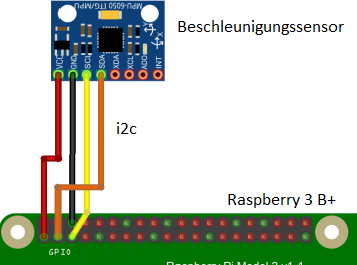
\includegraphics[width=0.33\textwidth]{Verkabelung_BeschlSensor}
    \caption{Verkabelung Beschleunigungssensor (http://fritzing.org)}
    \label{fig:Beschleunigungssensor}
  \end{figure}
  \begin{center}
  \begin{tabular}{lll}
  Bezeichnung     & GPIO Port & MPU 6050 \\ \hline
  Stromversorgung & 3V3      & VCC      \\ \hline
  Ground          & GND      & GND      \\ \hline
  Daten          & SDA      & SDA       \\ \hline
  Clock          & SCL      & SCL       \\ \hline
  \end{tabular}
  \end{center}
\end{table}

Auf dem Zug findet der Sensor Platz zwischen unserem Kran und dem Abstellplatz für den Würfel. Bei der Montage wurde darauf geachtet, dass die x-Achse Richtung Zugspitze zeigt und die y-Achse die Kräfte nach Links oder Rechts erfasst. Die z-Achse findet keine direkte Anwendung.

\paragraph{Prozessablauf}
Der Sensor wir für jede Achse separat angeschprochen, die erhaltenen Daten werden direkt das erste Mal umgewandelt. Sobald die 'Movement' Komponente gestartet wird, liest diese im 50ms Takt Daten über den Beschleunigungssensor ein. Die erhaltenen Daten werden ausgewertet und in Geschwindigkeit und Beschleunigung gerechnet.

\paragraph{Soll-Ist-Vergleich}
Die Messung der Beschleunigung erfolgt wie erwartet. Bei der Umrechnung herschen noch kleinere Unsicherheiten bezüglich der Genauigkeit.

\subsubsection{Entwicklungsablauf}
Es gibt es Vielzahl ähnlicher Beschleunigungssensoren auf dem Markt und somit auch mehr als genügend Bibliotheken auf dem Internet. Das Finden einer kompatiblen Bibliotheken erwies sich somit als eher trivial. Als nächstes wurde der Sensor an den GPIO Bus angeschlossen und mithilfe einer Testapplikation getestet. \\
Der Sensor reagierte jedoch nicht und so ging es weiter mit der Fehleranalyse. Nach dem Ausführen verschiedener anderer Applikationen und dem Austausch des Sensors wurde ich bald fündig. Wie sich heraustellte war das ganze nicht ganz so trivial wie gedacht und die Applikation muss auf Sensor, sowie GPIO angepasst werden. Ein Informatiker am Werk : )\\
Mit einem funktionierenden Sensor, konnte ich fortfahren und schrieb eine Klasse, welche den Sensor im 50ms Takt ausliest und weitergiebt. Die WebApp und die Middleware wurde noch entsprechend angepasst.\\

\subsubsection{Testing}
Anfangs wurde die Komponente über eine einfache Klasse mit Ausgabe auf ein Terminal Fenster getestet. Nach der Anbindung an das WebApp konnte die Beschleunigung jederzeit auf dem Web-Client angesehen werden. Eine plausibilisierung der erhaltenen Daten erfolgte nicht. Wir haben volles Vertrauen in den Sensor und die in der Applikation erfolgende Umrechnung.

\subsubsection{Reflexion}
Der Beschleunigungssensor ist eine interessante und im korrekten Einsatzgebiet sehr nützliche Komponente. Jedoch erhalten wir die Geschwindigkeit bereits vom Motor, somit haben wir redundante Daten bezüglich der Geschwindigkeit. Weil der Motor zuverlässigere Daten sendet, entschieden wir uns für den Weitergebrauch dieser Daten.

\end{document}